\chapter{Miniprojekt 3}
\section{Opgavebeskrivelse}
Opgaven lyder på at lave et selvvalgt projekt, som skal indeholde væsentlige elementer fra hele kurset. \\
Med udgangspunkt i ovenstående, er der valgt en opgave som lyder på følgende: \\
Analyser og sammenligne relevante analyser via filtre og FFT.
Til analysen er valgt et simpelt lydsignal hvor hhv. en kvinde siger "hello" og en mand siger "hello".\\ \\
Opgaven er valgt ud fra teorien om, at hvis der er mange harmoniske overtoner og få eller meget svage disharmoniske overtoner, lyder stemmen meget ren. Hvis billedet derimod er præget af mange kraftige, disharmoniske overtoner lyder stemmen uren eller hæs.
\newpage
\section{Analyse}
\subsection{Filtrering}
De to interessante figurere i denne case, er figur \ref{tidsdomaeet} og figur \ref{FFT Signal}. \\ Det ses på figur \ref{tidsdomaeet}, at begge signaler kører over ét sekund, hvorefter signalet er kortet ned til 0,6 sekunder, eftersom lyden befinder sig i intervallet herfra ned til 0.
\begin{figure}[H]
	\centering
	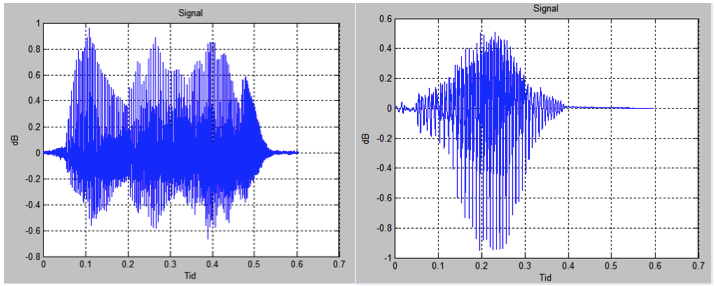
\includegraphics[width=1\textwidth]{Figurer/10}
	\caption{Signalt i tidsdomænet}
	\label{tidsdomaeet}
\end{figure}
Det ses her at damestemmen, figuren til venstre, bruger længere tid på at sige "hello", samt der i denne stemme er noget mere energi. \\ \\
På nedenstående figur (\ref{FFT Signal}), er der ud fra signalet foretaget en fourier transformation, således at der nu arbejdes i frekvensdomænet frem for tidsdomænet.
\begin{figure}[H]
	\centering
	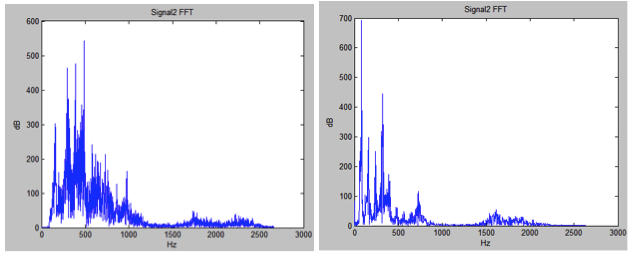
\includegraphics[width=1\textwidth]{Figurer/8}
	\caption{FFT Signal}
	\label{FFT Signal}
\end{figure}
Når man laver stemmeanalyse, kan man kigge på følgende punkter:
\begin{enumerate}
	\item Frekvensområde (Højeste frekvenser i spektret)
	\item Grundtone
	\item Overtoner
	\item Dominerende frekvens
\end{enumerate}
\textbf{Frekvensområde}
Frekvensområdet for kvindestemmet er fra ca. 100 Hz til 500 Hz, hvorimod ved mandestemmen er frekvensspektret fra ca. 50 Hz til ca. 400 Hz.\\ \\
\textbf{Grundtone}
For kvinde stemmen er ligger grundtonen ved 158 Hz, hvorimod ved mandestemmen, er grundtonen på 80 Hz. \\
\\
\textbf{Overtone}
Ved kvindestemmen er der tre overtoner: 292, 392 og 484, hvorimod ved mandestemmen er grundtonen den højeste og har altså ingen overtoner. Det at der er mange harmoniske overtoner ved kvindestemmen, viser at stemmen er meget ren. For mandestemmen er stemmen altså mere hæs.\\
\\
\textbf{Dominerende frekvens}
For kvindestemmen er den dominerende frekvens helt oppe på 484 Hz, hvor mandstemmens dominerende frekvens også er grundtonen.
Generelt er det tydeligt at damestemmen er lysere, mere klar og ren end mandestemmen, som er dybere og mere hæs/uren.

\subsection{Filtrering}
Yderligere er de to stemmer signaler filtreret, for at se om de forskellige filtre har indvirkning på hhv. kvinde og mandestemmer.
Først er der oprettet 3 filtre, et lavpas, båndpas og højpas filter, som gør sig gældende på begge signaler. Filtrenes knækfrekvenser er alle inden for det hørbare spektrum, eftersom analysen er af et hørbart lydsignal. Lavpas filtret er udformet som et IIR-filter, hvorimod båndpas og højpas er lavet som FIR-filter.\\Knækfrekvenserne er sat til:
\begin{itemize}
	\item Lavpas øvre = 7000
	\item Båndpas nedre = 6900
	\item Båndpas øvre = 14000
	\item Højpas nedre = 13900
\end{itemize}
Knækfrekvenserne overlapper med et med et lille interval, således at der ikke opstår dæmpninger eller forstærkninger, hvilket ses på figur \ref{Overlap}.\\
Først er der taget FFT af input signalet, for at finde impulsresponsen:

\begin{figure}[H]
	\centering
	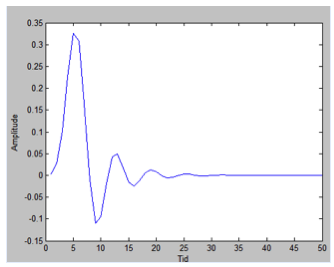
\includegraphics[width=0.7\textwidth]{Figurer/9}
	\caption{Signalimpuls}
	\label{Singalimpuls}
\end{figure}

Impulsresponsen er herefter brugt til udarbejdelse af IIR-lavpasfiltret:

\begin{figure}[H]
	\centering
	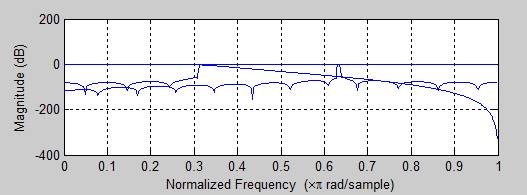
\includegraphics[width=1\textwidth]{Figurer/3}
	\caption{Overlap}
	\label{Overlap}
\end{figure}

I lavpas filtret ses hvordan de høje frekvenser dør ud, og hvilke lave frekvenser der lukkes igennem:

\begin{figure}[H]
	\centering
	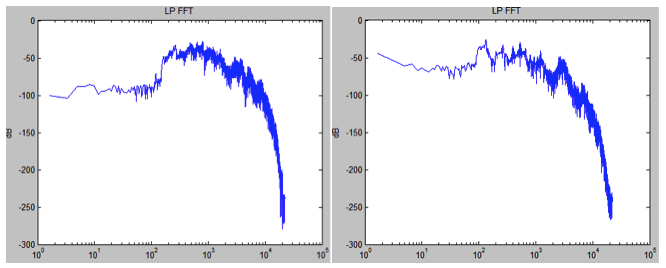
\includegraphics[width=1\textwidth]{Figurer/2}
	\caption{FFT lavpas}
	\label{FFT signal}
\end{figure}

I båndpasfiltret ses at forstærkningen stemmer overens med knækfrekvensen, og man på den måde kan manipulere med stemmesignalet:

\begin{figure}[H]
	\centering
	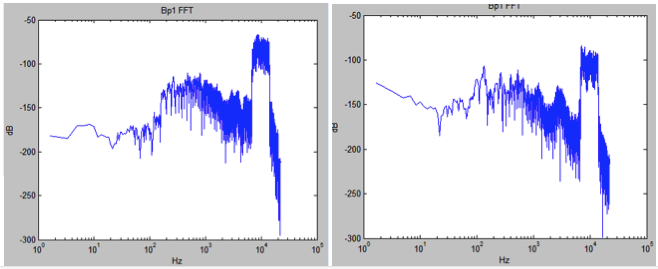
\includegraphics[width=1\textwidth]{Figurer/5}
	\caption{FFT båndpas}
	\label{FFT baandpas}
\end{figure}

Højpasfiltret ses det hvilke højefrekvenser der lukkes ingennem:

\begin{figure}[H]
	\centering
	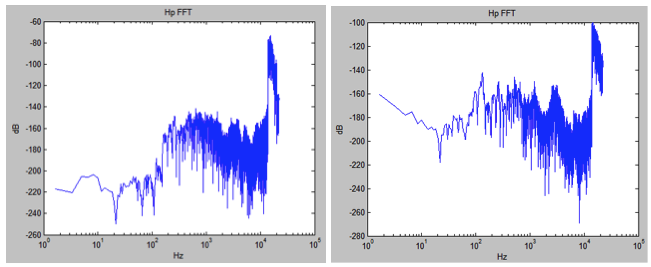
\includegraphics[width=1\textwidth]{Figurer/6}
	\caption{FFT højpas}
	\label{FFT hoejpas}
\end{figure}

\section{Konklusion}
Ved hjælp af digital signal behandling, kan man analysere stemmer og hermed se tydelige forskelle på mande- og kvindestemmer. Yderligere kan man også manipulere med stemmerne, ved at filtrere signalerne.



